\begin{center}
    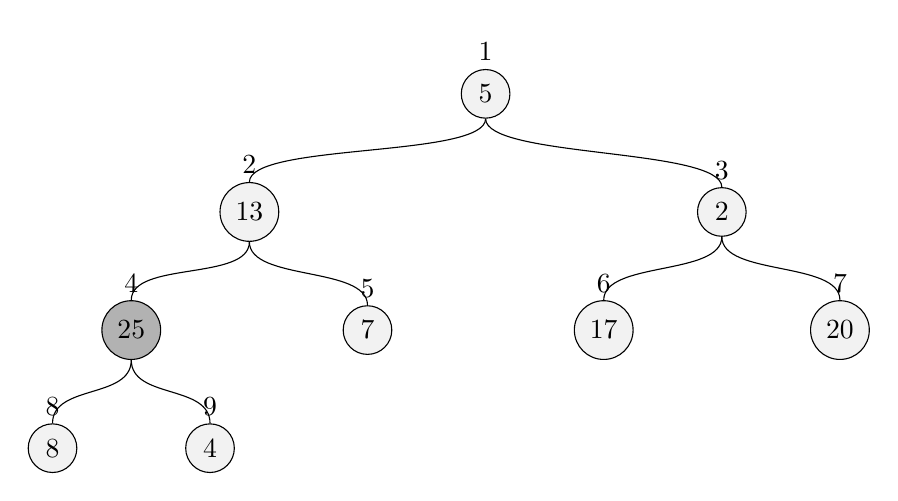
\begin{tikzpicture}[
       edge from parent path=
    {(\tikzparentnode.south) .. controls +(0,-.5) and +(0,.5)
                             .. (\tikzchildnode.north)},
    level 1/.style={sibling distance=6cm}, 
    level 2/.style={sibling distance=3cm},                        
    level 3/.style={sibling distance=2cm},                         
    level 4/.style={sibling distance=1cm},
   every node/.style={draw, circle, fill=gray, fill opacity=0.1, text opacity=1},
   label distance=-1mm]
   
\node[label=90:$1$] {5}
    child {node[label=90:$2$] {13}
        child {node[label=90:$4$, fill=black, fill opacity=0.3] {25}
            child {node[label=90:$8$] {8}}
            child {node[label=90:$9$] {4}}
        }
        child {node[label=90:$5$] {7}}
    }
    child {node[label=90:$3$] {2}
        child {node[label=90:$6$] {17}}
        child {node[label=90:$7$] {20}}
    };

\end{tikzpicture}
\end{center}

\begin{center}
    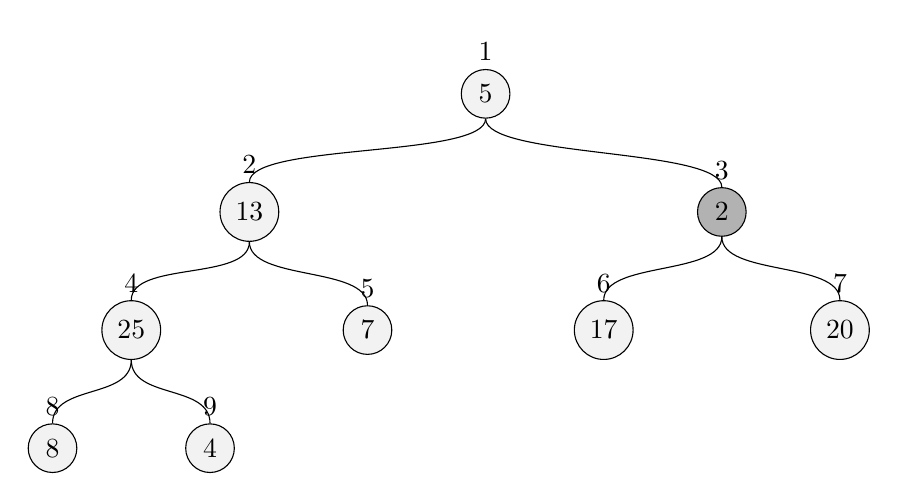
\begin{tikzpicture}[
       edge from parent path=
    {(\tikzparentnode.south) .. controls +(0,-.5) and +(0,.5)
                             .. (\tikzchildnode.north)},
    level 1/.style={sibling distance=6cm}, 
    level 2/.style={sibling distance=3cm},                        
    level 3/.style={sibling distance=2cm},                         
    level 4/.style={sibling distance=1cm},
   every node/.style={draw, circle, fill=gray, fill opacity=0.1, text opacity=1},
   label distance=-1mm]
   
\node[label=90:$1$] {5}
    child {node[label=90:$2$] {13}
        child {node[label=90:$4$] {25}
            child {node[label=90:$8$] {8}}
            child {node[label=90:$9$] {4}}
        }
        child {node[label=90:$5$] {7}}
    }
    child {node[label=90:$3$, fill=black, fill opacity=0.3] {2}
        child {node[label=90:$6$] {17}}
        child {node[label=90:$7$] {20}}
    };

\end{tikzpicture}
\end{center}

\begin{center}
    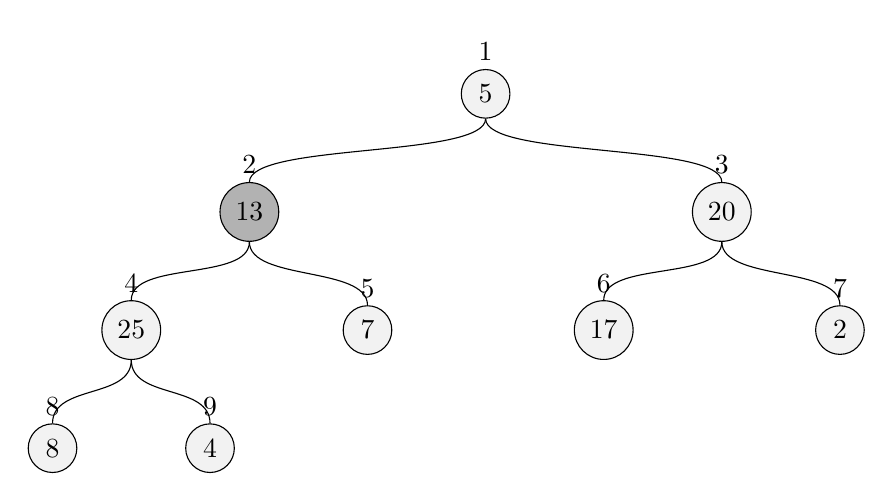
\begin{tikzpicture}[
       edge from parent path=
    {(\tikzparentnode.south) .. controls +(0,-.5) and +(0,.5)
                             .. (\tikzchildnode.north)},
    level 1/.style={sibling distance=6cm}, 
    level 2/.style={sibling distance=3cm},                        
    level 3/.style={sibling distance=2cm},                         
    level 4/.style={sibling distance=1cm},
   every node/.style={draw, circle, fill=gray, fill opacity=0.1, text opacity=1},
   label distance=-1mm]
   
\node[label=90:$1$] {5}
    child {node[label=90:$2$, fill=black, fill opacity=0.3] {13}
        child {node[label=90:$4$] {25}
            child {node[label=90:$8$] {8}}
            child {node[label=90:$9$] {4}}
        }
        child {node[label=90:$5$] {7}}
    }
    child {node[label=90:$3$] {20}
        child {node[label=90:$6$] {17}}
        child {node[label=90:$7$] {2}}
    };

\end{tikzpicture}
\end{center}

\begin{center}
    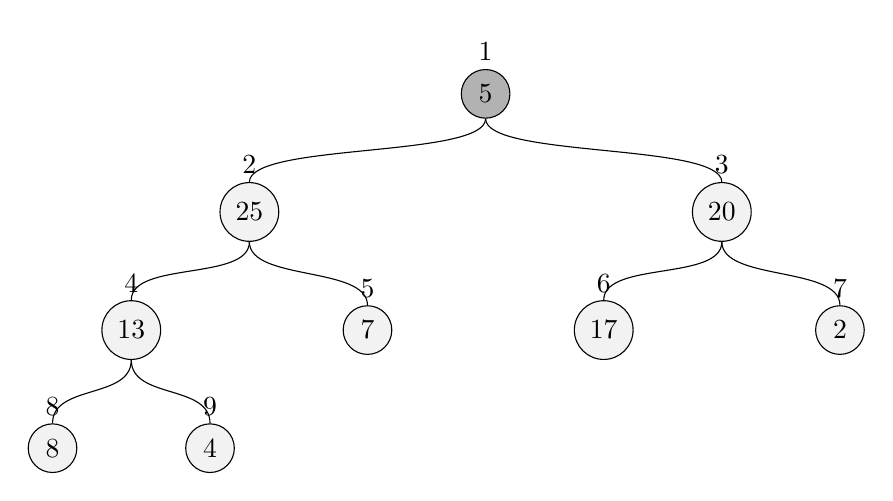
\begin{tikzpicture}[
       edge from parent path=
    {(\tikzparentnode.south) .. controls +(0,-.5) and +(0,.5)
                             .. (\tikzchildnode.north)},
    level 1/.style={sibling distance=6cm}, 
    level 2/.style={sibling distance=3cm},                        
    level 3/.style={sibling distance=2cm},                         
    level 4/.style={sibling distance=1cm},
   every node/.style={draw, circle, fill=gray, fill opacity=0.1, text opacity=1},
   label distance=-1mm]
   
\node[label=90:$1$, fill=black, fill opacity=0.3] {5}
    child {node[label=90:$2$] {25}
        child {node[label=90:$4$] {13}
            child {node[label=90:$8$] {8}}
            child {node[label=90:$9$] {4}}
        }
        child {node[label=90:$5$] {7}}
    }
    child {node[label=90:$3$] {20}
        child {node[label=90:$6$] {17}}
        child {node[label=90:$7$] {2}}
    };

\end{tikzpicture}
\end{center}

\begin{center}
    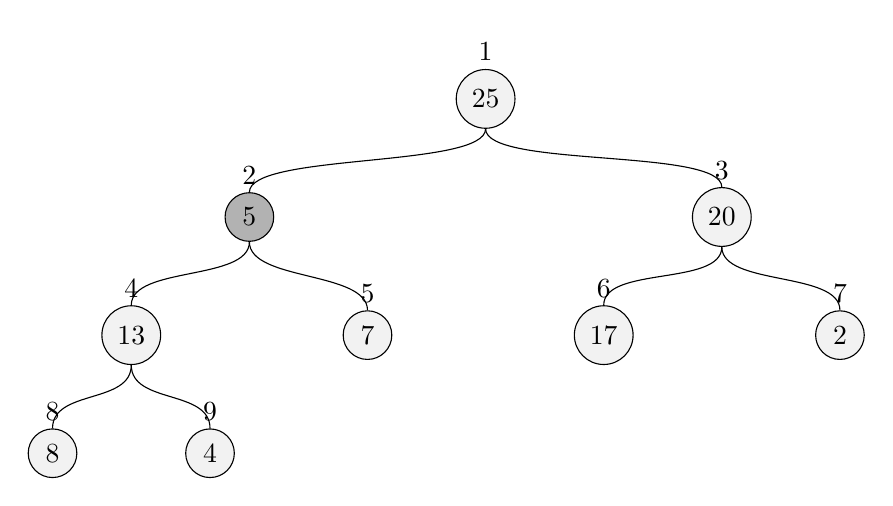
\begin{tikzpicture}[
       edge from parent path=
    {(\tikzparentnode.south) .. controls +(0,-.5) and +(0,.5)
                             .. (\tikzchildnode.north)},
    level 1/.style={sibling distance=6cm}, 
    level 2/.style={sibling distance=3cm},                        
    level 3/.style={sibling distance=2cm},                         
    level 4/.style={sibling distance=1cm},
   every node/.style={draw, circle, fill=gray, fill opacity=0.1, text opacity=1},
   label distance=-1mm]
   
\node[label=90:$1$] {25}
    child {node[label=90:$2$, fill=black, fill opacity=0.3] {5}
        child {node[label=90:$4$] {13}
            child {node[label=90:$8$] {8}}
            child {node[label=90:$9$] {4}}
        }
        child {node[label=90:$5$] {7}}
    }
    child {node[label=90:$3$] {20}
        child {node[label=90:$6$] {17}}
        child {node[label=90:$7$] {2}}
    };

\end{tikzpicture}
\end{center}

\begin{center}
    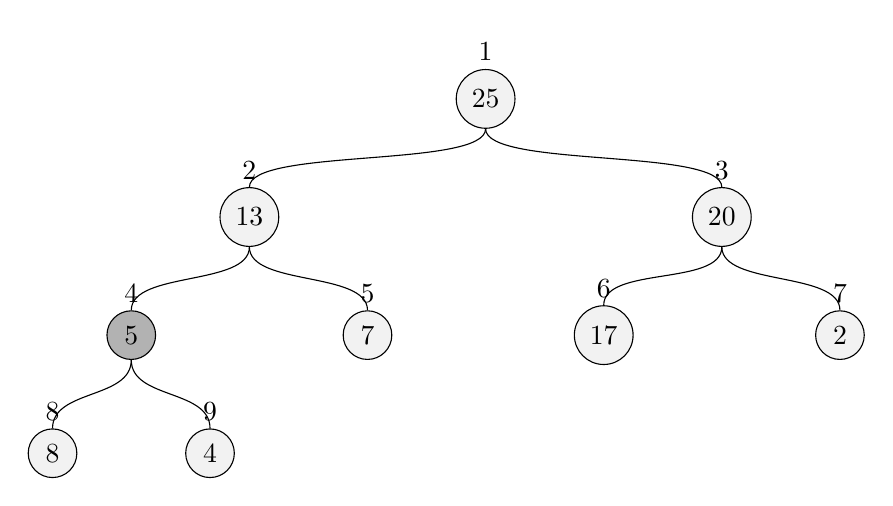
\begin{tikzpicture}[
       edge from parent path=
    {(\tikzparentnode.south) .. controls +(0,-.5) and +(0,.5)
                             .. (\tikzchildnode.north)},
    level 1/.style={sibling distance=6cm}, 
    level 2/.style={sibling distance=3cm},                        
    level 3/.style={sibling distance=2cm},                         
    level 4/.style={sibling distance=1cm},
   every node/.style={draw, circle, fill=gray, fill opacity=0.1, text opacity=1},
   label distance=-1mm]
   
\node[label=90:$1$] {25}
    child {node[label=90:$2$] {13}
        child {node[label=90:$4$, fill=black, fill opacity=0.3] {5}
            child {node[label=90:$8$] {8}}
            child {node[label=90:$9$] {4}}
        }
        child {node[label=90:$5$] {7}}
    }
    child {node[label=90:$3$] {20}
        child {node[label=90:$6$] {17}}
        child {node[label=90:$7$] {2}}
    };

\end{tikzpicture}
\end{center}

\begin{center}
    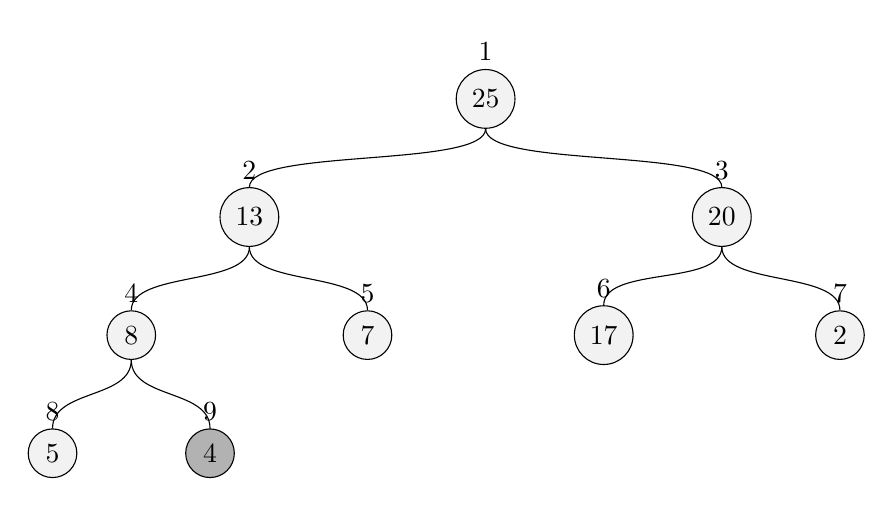
\begin{tikzpicture}[
       edge from parent path=
    {(\tikzparentnode.south) .. controls +(0,-.5) and +(0,.5)
                             .. (\tikzchildnode.north)},
    level 1/.style={sibling distance=6cm}, 
    level 2/.style={sibling distance=3cm},                        
    level 3/.style={sibling distance=2cm},                         
    level 4/.style={sibling distance=1cm},
   every node/.style={draw, circle, fill=gray, fill opacity=0.1, text opacity=1},
   label distance=-1mm]
   
\node[label=90:$1$] {25}
    child {node[label=90:$2$] {13}
        child {node[label=90:$4$] {8}
            child {node[label=90:$8$] {5}}
            child {node[label=90:$9$, fill=black, fill opacity=0.3] {4}}
        }
        child {node[label=90:$5$] {7}}
    }
    child {node[label=90:$3$] {20}
        child {node[label=90:$6$] {17}}
        child {node[label=90:$7$] {2}}
    };

\end{tikzpicture}
\end{center}

% Start heapsort

\begin{center}
    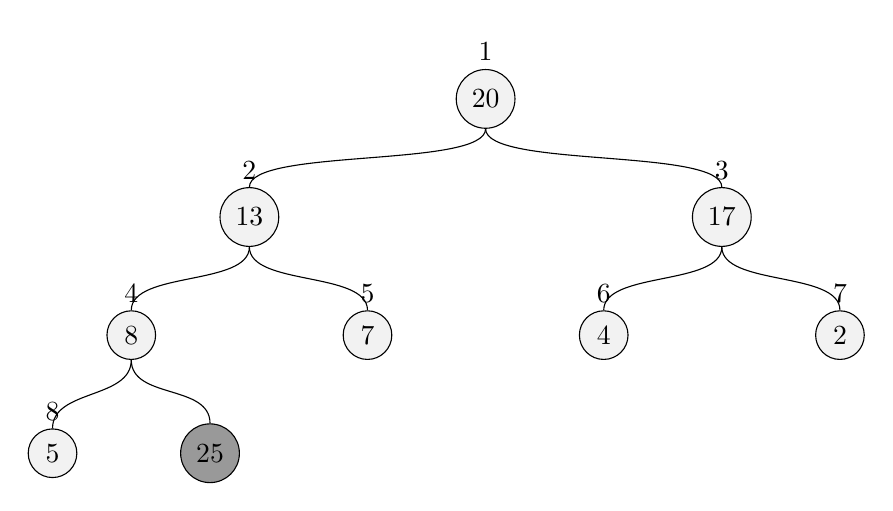
\begin{tikzpicture}[
       edge from parent path=
    {(\tikzparentnode.south) .. controls +(0,-.5) and +(0,.5)
                             .. (\tikzchildnode.north)},
    level 1/.style={sibling distance=6cm}, 
    level 2/.style={sibling distance=3cm},                        
    level 3/.style={sibling distance=2cm},                         
    level 4/.style={sibling distance=1cm},
   every node/.style={draw, circle, fill=gray, fill opacity=0.1, text opacity=1},
   label distance=-1mm]
   
\node[label=90:$1$] {20}
    child {node[label=90:$2$] {13}
        child {node[label=90:$4$] {8}
            child {node[label=90:$8$] {5}}
            child {node[fill=black, fill opacity=0.4] {25}}
        }
        child {node[label=90:$5$] {7}}
    }
    child {node[label=90:$3$] {17}
        child {node[label=90:$6$] {4}}
        child {node[label=90:$7$] {2}}
    };

\end{tikzpicture}
\end{center}

\begin{center}
    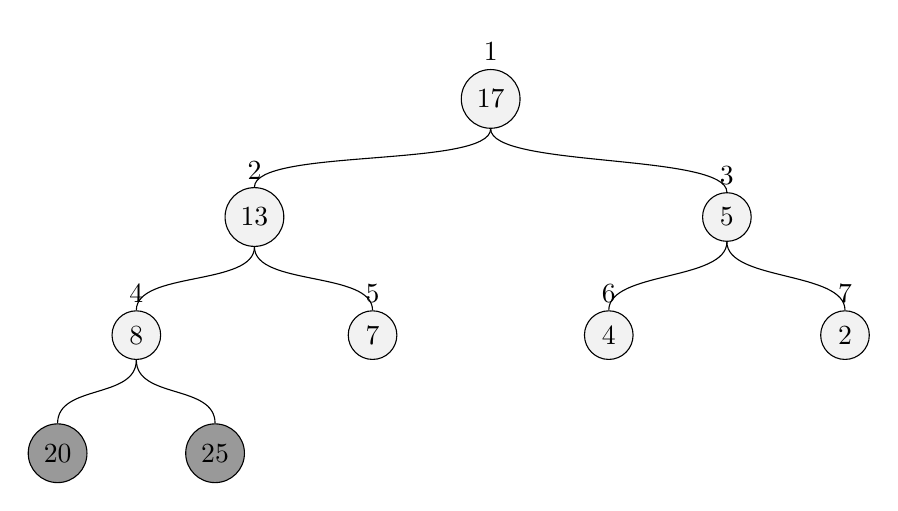
\begin{tikzpicture}[
       edge from parent path=
    {(\tikzparentnode.south) .. controls +(0,-.5) and +(0,.5)
                             .. (\tikzchildnode.north)},
    level 1/.style={sibling distance=6cm}, 
    level 2/.style={sibling distance=3cm},                        
    level 3/.style={sibling distance=2cm},                         
    level 4/.style={sibling distance=1cm},
   every node/.style={draw, circle, fill=gray, fill opacity=0.1, text opacity=1},
   label distance=-1mm]
   
\node[label=90:$1$] {17}
    child {node[label=90:$2$] {13}
        child {node[label=90:$4$] {8}
            child {node[fill=black, fill opacity=0.4] {20}}
            child {node[fill=black, fill opacity=0.4] {25}}
        }
        child {node[label=90:$5$] {7}}
    }
    child {node[label=90:$3$] {5}
        child {node[label=90:$6$] {4}}
        child {node[label=90:$7$] {2}}
    };

\end{tikzpicture}
\end{center}

\begin{center}
    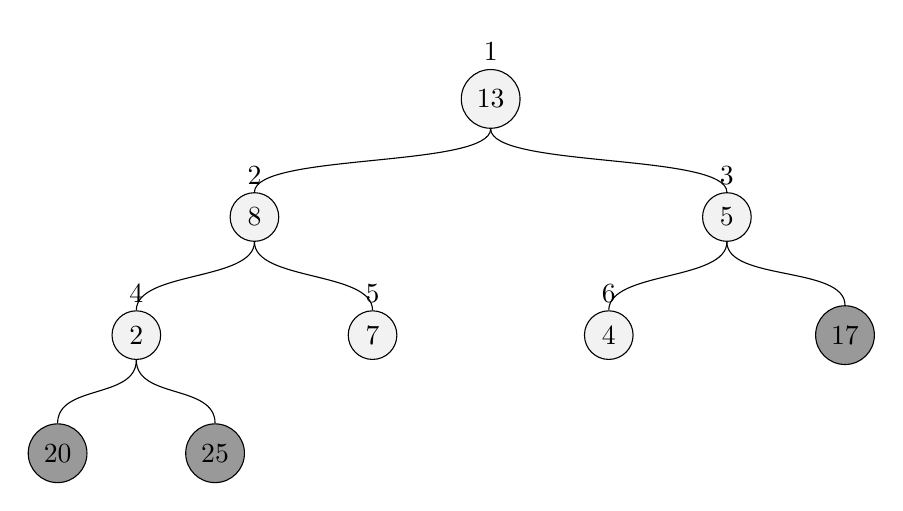
\begin{tikzpicture}[
       edge from parent path=
    {(\tikzparentnode.south) .. controls +(0,-.5) and +(0,.5)
                             .. (\tikzchildnode.north)},
    level 1/.style={sibling distance=6cm}, 
    level 2/.style={sibling distance=3cm},                        
    level 3/.style={sibling distance=2cm},                         
    level 4/.style={sibling distance=1cm},
   every node/.style={draw, circle, fill=gray, fill opacity=0.1, text opacity=1},
   label distance=-1mm]
   
\node[label=90:$1$] {13}
    child {node[label=90:$2$] {8}
        child {node[label=90:$4$] {2}
            child {node[fill=black, fill opacity=0.4] {20}}
            child {node[fill=black, fill opacity=0.4] {25}}
        }
        child {node[label=90:$5$] {7}}
    }
    child {node[label=90:$3$] {5}
        child {node[label=90:$6$] {4}}
        child {node[fill=black, fill opacity=0.4] {17}}
    };

\end{tikzpicture}
\end{center}

\begin{center}
    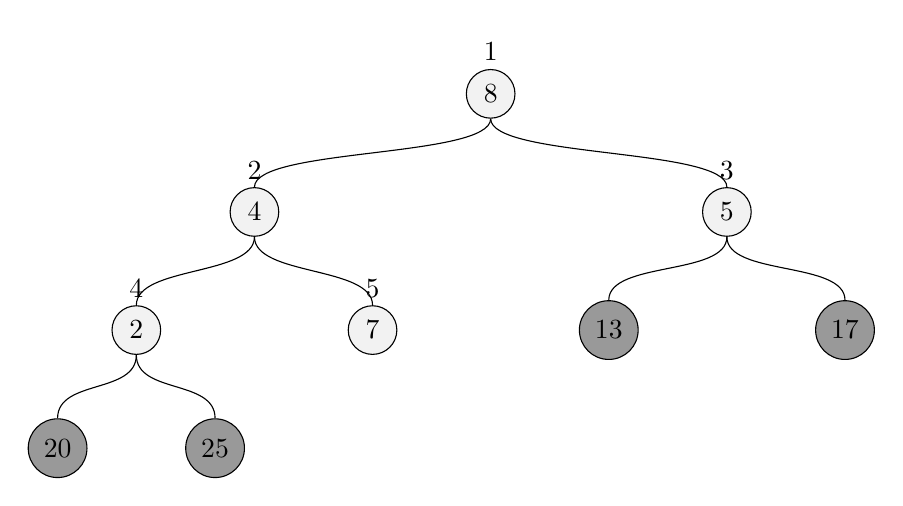
\begin{tikzpicture}[
       edge from parent path=
    {(\tikzparentnode.south) .. controls +(0,-.5) and +(0,.5)
                             .. (\tikzchildnode.north)},
    level 1/.style={sibling distance=6cm}, 
    level 2/.style={sibling distance=3cm},                        
    level 3/.style={sibling distance=2cm},                         
    level 4/.style={sibling distance=1cm},
   every node/.style={draw, circle, fill=gray, fill opacity=0.1, text opacity=1},
   label distance=-1mm]
   
\node[label=90:$1$] {8}
    child {node[label=90:$2$] {4}
        child {node[label=90:$4$] {2}
            child {node[fill=black, fill opacity=0.4] {20}}
            child {node[fill=black, fill opacity=0.4] {25}}
        }
        child {node[label=90:$5$] {7}}
    }
    child {node[label=90:$3$] {5}
        child {node[fill=black, fill opacity=0.4] {13}}
        child {node[fill=black, fill opacity=0.4] {17}}
    };

\end{tikzpicture}
\end{center}

\begin{center}
    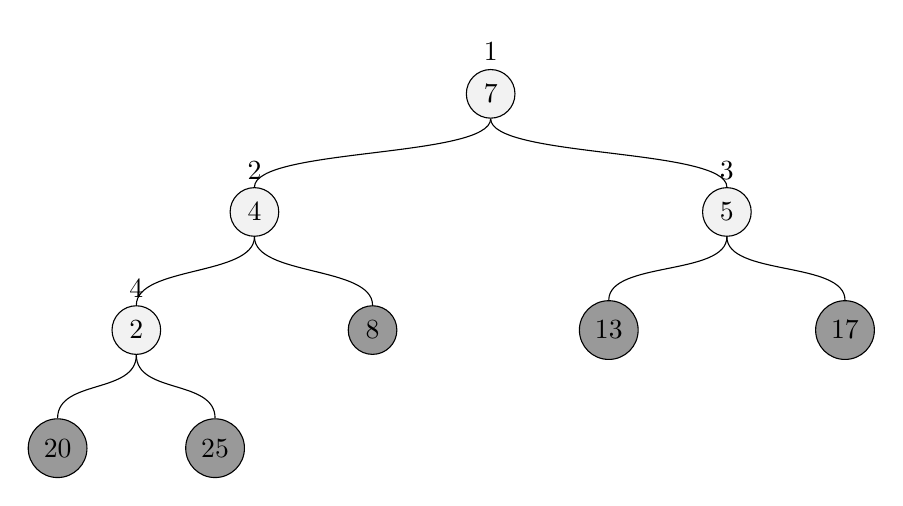
\begin{tikzpicture}[
       edge from parent path=
    {(\tikzparentnode.south) .. controls +(0,-.5) and +(0,.5)
                             .. (\tikzchildnode.north)},
    level 1/.style={sibling distance=6cm}, 
    level 2/.style={sibling distance=3cm},                        
    level 3/.style={sibling distance=2cm},                         
    level 4/.style={sibling distance=1cm},
   every node/.style={draw, circle, fill=gray, fill opacity=0.1, text opacity=1},
   label distance=-1mm]
   
\node[label=90:$1$] {7}
    child {node[label=90:$2$] {4}
        child {node[label=90:$4$] {2}
            child {node[fill=black, fill opacity=0.4] {20}}
            child {node[fill=black, fill opacity=0.4] {25}}
        }
        child {node[fill=black, fill opacity=0.4] {8}}
    }
    child {node[label=90:$3$] {5}
        child {node[fill=black, fill opacity=0.4] {13}}
        child {node[fill=black, fill opacity=0.4] {17}}
    };

\end{tikzpicture}
\end{center}

\begin{center}
    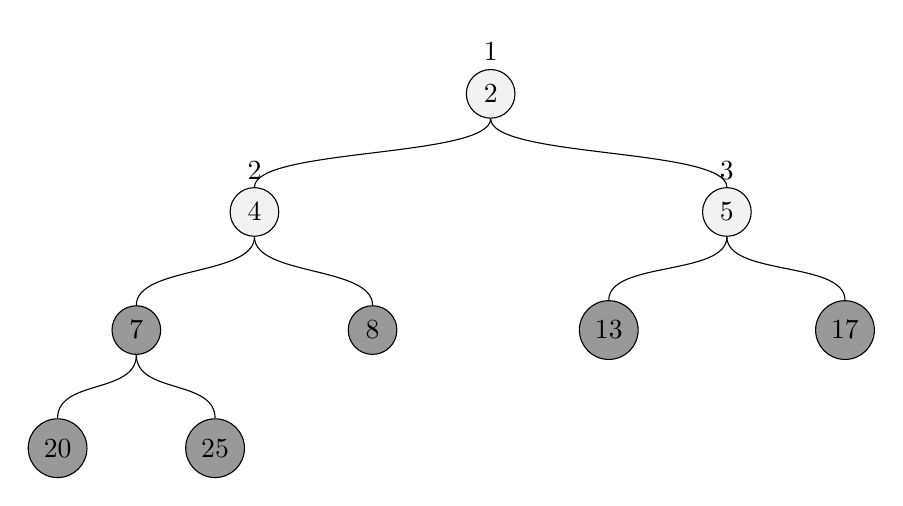
\begin{tikzpicture}[
       edge from parent path=
    {(\tikzparentnode.south) .. controls +(0,-.5) and +(0,.5)
                             .. (\tikzchildnode.north)},
    level 1/.style={sibling distance=6cm}, 
    level 2/.style={sibling distance=3cm},                        
    level 3/.style={sibling distance=2cm},                         
    level 4/.style={sibling distance=1cm},
   every node/.style={draw, circle, fill=gray, fill opacity=0.1, text opacity=1},
   label distance=-1mm]
   
\node[label=90:$1$] {2}
    child {node[label=90:$2$] {4}
        child {node[fill=black, fill opacity=0.4] {7}
            child {node[fill=black, fill opacity=0.4] {20}}
            child {node[fill=black, fill opacity=0.4] {25}}
        }
        child {node[fill=black, fill opacity=0.4] {8}}
    }
    child {node[label=90:$3$] {5}
        child {node[fill=black, fill opacity=0.4] {13}}
        child {node[fill=black, fill opacity=0.4] {17}}
    };

\end{tikzpicture}
\end{center}

\begin{center}
    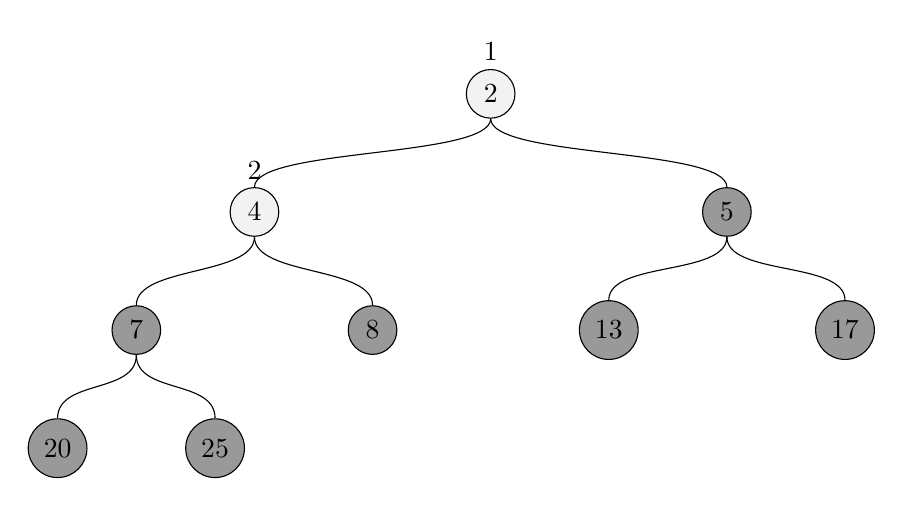
\begin{tikzpicture}[
       edge from parent path=
    {(\tikzparentnode.south) .. controls +(0,-.5) and +(0,.5)
                             .. (\tikzchildnode.north)},
    level 1/.style={sibling distance=6cm}, 
    level 2/.style={sibling distance=3cm},                        
    level 3/.style={sibling distance=2cm},                         
    level 4/.style={sibling distance=1cm},
   every node/.style={draw, circle, fill=gray, fill opacity=0.1, text opacity=1},
   label distance=-1mm]
   
\node[label=90:$1$] {2}
    child {node[label=90:$2$] {4}
        child {node[fill=black, fill opacity=0.4] {7}
            child {node[fill=black, fill opacity=0.4] {20}}
            child {node[fill=black, fill opacity=0.4] {25}}
        }
        child {node[fill=black, fill opacity=0.4] {8}}
    }
    child {node[fill=black, fill opacity=0.4] {5}
        child {node[fill=black, fill opacity=0.4] {13}}
        child {node[fill=black, fill opacity=0.4] {17}}
    };

\end{tikzpicture}
\end{center}

\begin{center}
    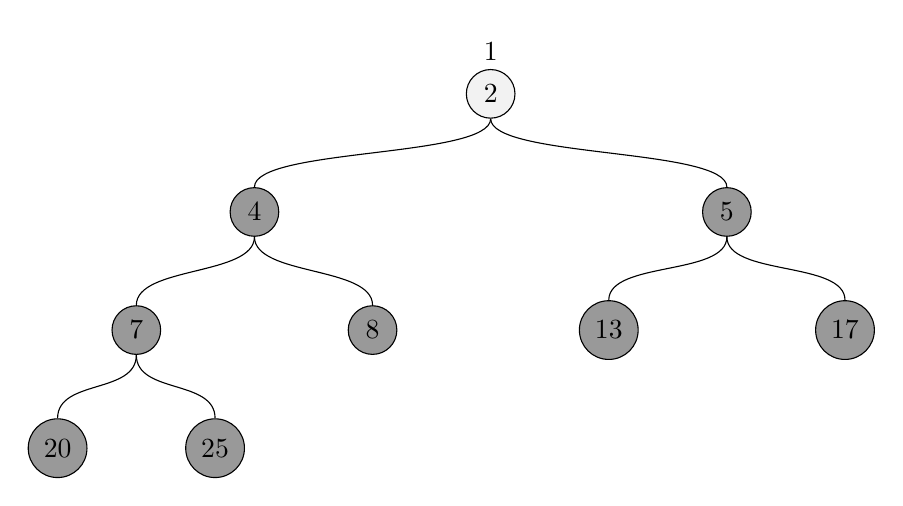
\begin{tikzpicture}[
       edge from parent path=
    {(\tikzparentnode.south) .. controls +(0,-.5) and +(0,.5)
                             .. (\tikzchildnode.north)},
    level 1/.style={sibling distance=6cm}, 
    level 2/.style={sibling distance=3cm},                        
    level 3/.style={sibling distance=2cm},                         
    level 4/.style={sibling distance=1cm},
   every node/.style={draw, circle, fill=gray, fill opacity=0.1, text opacity=1},
   label distance=-1mm]
   
\node[label=90:$1$] {2}
    child {node[fill=black, fill opacity=0.4] {4}
        child {node[fill=black, fill opacity=0.4] {7}
            child {node[fill=black, fill opacity=0.4] {20}}
            child {node[fill=black, fill opacity=0.4] {25}}
        }
        child {node[fill=black, fill opacity=0.4] {8}}
    }
    child {node[fill=black, fill opacity=0.4] {5}
        child {node[fill=black, fill opacity=0.4] {13}}
        child {node[fill=black, fill opacity=0.4] {17}}
    };

\end{tikzpicture}
\end{center}

\begin{center}
    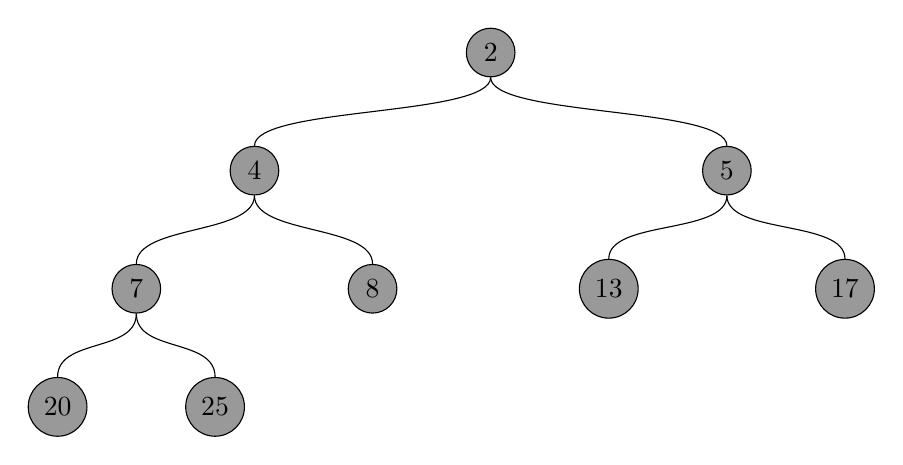
\begin{tikzpicture}[
       edge from parent path=
    {(\tikzparentnode.south) .. controls +(0,-.5) and +(0,.5)
                             .. (\tikzchildnode.north)},
    level 1/.style={sibling distance=6cm}, 
    level 2/.style={sibling distance=3cm},                        
    level 3/.style={sibling distance=2cm},                         
    level 4/.style={sibling distance=1cm},
   every node/.style={draw, circle, fill=gray, fill opacity=0.1, text opacity=1},
   label distance=-1mm]
   
\node[fill=black, fill opacity=0.4] {2}
    child {node[fill=black, fill opacity=0.4] {4}
        child {node[fill=black, fill opacity=0.4] {7}
            child {node[fill=black, fill opacity=0.4] {20}}
            child {node[fill=black, fill opacity=0.4] {25}}
        }
        child {node[fill=black, fill opacity=0.4] {8}}
    }
    child {node[fill=black, fill opacity=0.4] {5}
        child {node[fill=black, fill opacity=0.4] {13}}
        child {node[fill=black, fill opacity=0.4] {17}}
    };

\end{tikzpicture}
\end{center}

\begin{center}
    \begin{tikzpicture}[
        start chain = going right, node distance = 0pt, 
        every node/.style={draw, minimum width=2em, minimum height=2em,
                            outer sep=0pt, on chain, fill=gray, fill opacity=0.2, text opacity=1},
        ]
    \node[] {$2$};
    \node[] {$4$};
    \node[] {$5$};
    \node[] {$7$};
    \node[] {$8$};
    \node[] {$13$};
    \node[] {$17$};
    \node[] {$20$};
    \node[] {$25$};
    \end{tikzpicture}
\end{center}